\documentclass{article}\usepackage[]{graphicx}\usepackage[]{color}
% maxwidth is the original width if it is less than linewidth
% otherwise use linewidth (to make sure the graphics do not exceed the margin)
\makeatletter
\def\maxwidth{ %
  \ifdim\Gin@nat@width>\linewidth
    \linewidth
  \else
    \Gin@nat@width
  \fi
}
\makeatother

\definecolor{fgcolor}{rgb}{0.345, 0.345, 0.345}
\newcommand{\hlnum}[1]{\textcolor[rgb]{0.686,0.059,0.569}{#1}}%
\newcommand{\hlstr}[1]{\textcolor[rgb]{0.192,0.494,0.8}{#1}}%
\newcommand{\hlcom}[1]{\textcolor[rgb]{0.678,0.584,0.686}{\textit{#1}}}%
\newcommand{\hlopt}[1]{\textcolor[rgb]{0,0,0}{#1}}%
\newcommand{\hlstd}[1]{\textcolor[rgb]{0.345,0.345,0.345}{#1}}%
\newcommand{\hlkwa}[1]{\textcolor[rgb]{0.161,0.373,0.58}{\textbf{#1}}}%
\newcommand{\hlkwb}[1]{\textcolor[rgb]{0.69,0.353,0.396}{#1}}%
\newcommand{\hlkwc}[1]{\textcolor[rgb]{0.333,0.667,0.333}{#1}}%
\newcommand{\hlkwd}[1]{\textcolor[rgb]{0.737,0.353,0.396}{\textbf{#1}}}%
\let\hlipl\hlkwb

\usepackage{framed}
\makeatletter
\newenvironment{kframe}{%
 \def\at@end@of@kframe{}%
 \ifinner\ifhmode%
  \def\at@end@of@kframe{\end{minipage}}%
  \begin{minipage}{\columnwidth}%
 \fi\fi%
 \def\FrameCommand##1{\hskip\@totalleftmargin \hskip-\fboxsep
 \colorbox{shadecolor}{##1}\hskip-\fboxsep
     % There is no \\@totalrightmargin, so:
     \hskip-\linewidth \hskip-\@totalleftmargin \hskip\columnwidth}%
 \MakeFramed {\advance\hsize-\width
   \@totalleftmargin\z@ \linewidth\hsize
   \@setminipage}}%
 {\par\unskip\endMakeFramed%
 \at@end@of@kframe}
\makeatother

\definecolor{shadecolor}{rgb}{.97, .97, .97}
\definecolor{messagecolor}{rgb}{0, 0, 0}
\definecolor{warningcolor}{rgb}{1, 0, 1}
\definecolor{errorcolor}{rgb}{1, 0, 0}
\newenvironment{knitrout}{}{} % an empty environment to be redefined in TeX

\usepackage{alltt}
\usepackage{Sweave}
\usepackage{float}
\usepackage{graphicx}
\usepackage{tabularx}
\usepackage{siunitx}
\usepackage{amssymb} % for math symbols
\usepackage{amsmath} % for aligning equations
\usepackage{textcomp}
\usepackage{url}
\usepackage{mdframed}
\usepackage[T1]{fontenc}
\usepackage{subcaption}
\usepackage{natbib}
\bibliographystyle{..//refs/styles/besjournals.bst}
\usepackage[small]{caption}
\setlength{\captionmargin}{30pt}
\setlength{\abovecaptionskip}{0pt}
\setlength{\belowcaptionskip}{10pt}
\captionsetup{justification=raggedright,singlelinecheck=false}
\topmargin -1.5cm        
\oddsidemargin -0.04cm   
\evensidemargin -0.04cm
\textwidth 16.59cm
\textheight 21.94cm 
%\pagestyle{empty} %comment if want page numbers
\parskip 7.2pt
\renewcommand{\baselinestretch}{1.5}
\parindent 0pt
\usepackage{lineno}
\linenumbers

%cross referencing:
\usepackage{xr}
\usepackage{xr-hyper}
\externaldocument{micro_supp}

\newmdenv[
  topline=true,
  bottomline=true,
  skipabove=\topsep,
  skipbelow=\topsep
]{siderules}
\IfFileExists{upquote.sty}{\usepackage{upquote}}{}
\begin{document}

\noindent\textbf{\Large{Comparing spring phenology in an urban arboretum versus rural forested site and implications for forecasting}}

\noindent Authors:\\
C. J. Chamberlain $^{1,2}$ \& E. M. Wolkovich $^{1,2,3}$
\vspace{2ex}\\
\emph{Author affiliations:}\\
$^{1}$Arnold Arboretum of Harvard University, 1300 Centre Street, Boston, Massachusetts, USA; \\
$^{2}$Organismic \& Evolutionary Biology, Harvard University, 26 Oxford Street, Cambridge, Massachusetts, USA; \\
$^{3}$Forest \& Conservation Sciences, Faculty of Forestry, University of British Columbia, 2424 Main Mall, Vancouver, BC V6T 1Z4\\
\vspace{2ex}
$^*$Corresponding author: 248.953.0189; cchamberlain@g.harvard.edu\\

\noindent \emph{Keywords:} phenology, climate change, forest communities, microclimate, urban heat island, growing degree days\\

\renewcommand{\thetable}{\arabic{table}}
\renewcommand{\thefigure}{\arabic{figure}}
\renewcommand{\labelitemi}{$-$}
\setkeys{Gin}{width=0.8\textwidth}

%%%%%%%%%%%%%%%%%%%%%%%%%%%%%%%%%%%%%%%%%%%%%%%
%%%%%%%%%%%%%%%%%%%%%%%%%%%%%%%%%%%%%%%%%%%%%%%


\newpage
\section*{Abstract} 
Predicting spring plant phenology in temperate forests is critical for forecasting important processes such as carbon storage, especially as climate change and urbanization shift many phenological phases. One major forecasting method for phenology is the growing degree day (GDD) model, which tracks heat accumulation. GDD models typically assume that the GDD threshold for a species, or even functional type, is constant across diverse landscapes, but increasing evidence suggests otherwise. Shifts in climate, especially warmer winters, may alter the required GDD. As climate can vary on small spatial scales---and recent studies suggest that fine-scale climate may matter to phenology---GDD requirements may vary importantly across space. Here, we use simulations and observations from one urban arboretum and one rural forested site to assess how consistent GDD models of budburst are across species and landscapes. Additionally, we compare two methods to measure climate data (i.e., weather station data and hobo logger data). Our results suggest the urban arboretum site requires fewer GDDs until budburst and may have stronger microclimate effects than the rural forested site though these effects diminish with the use of hobo loggers. We also find that GDD models may become less accurate with warming as GDDs begin to accumulate faster. Our findings suggest we may need to either use a method that is less reliant on accumulated, climatological sums or we must scrutinize results through the use of mixed models and simulated data.

\section*{Introduction}

Understanding and predicting spring plant phenology in temperate deciduous forests is critical as it both shapes community structure and also influences major ecosystem services such as resource and forest management. Climate change and urbanization are advancing spring timing---such as budburst and leafout, which are strongly cued by temperature, resulting in longer growing seasons \citep{Chuine2001}. These shifts in growing seasons ultimately impact ecosystem services. Spring budburst timing in particular can have cascading effects on pollinators \citep{Boggs2012, Pardee2017}, albedo \citep{Williamson2016}, and carbon dynamics \citep{Richardson2013}. Temperate forests sequester carbon and help mitigate the negative effects of climate change and---with earlier spring phenology and longer growing seasons---there has been an increase in carbon uptake \citep{Keenan2014}. Because of the importance of phenology, forecasting it accurately with climate change is a major and important aim across several fields of science including agronomy, ecology, evolution and hydrology \citep{Moorcroft2001,Bolton2013,Yu2016,Taylor2020}. 
  
One major forecasting method across all these fields is the growing degree day model. The growing degree day (GDD) model allows researchers to track heat accumulation to predict spring budburst \citep{Schwartz2006,Vitasse2011,Cook2012,Phillimore2013,Crimmins2020}. The GDD model simply sums temperatures above a certain threshold---often 0$^{\circ}$C for forest trees  \citep[as estimates are proven to be more accurate,][]{Man2010}---and different species often require a different number of GDDs to leaf out. GDDs accumulate at a faster rate when mean temperatures are higher, thus different sites or different climate measurement methods may record different GDD thresholds for budburst. Understanding the intricacies of the GDD model is essential for predicting the effects of climate change on systems where the climate is rapidly changing, including temperate forests. 
  
We often assume in GDD models that the GDD required for a species, or even a suite of species (e.g., plant functional types) is constant, but increasing evidence suggests it may not be. The plasticity of phenology means that the same individual exposed to different climates will leafout at a very different time. Decades of work show that chilling---related to winter temperatures---and photoperiod can shift the GDD a plant needs for the same event \citep{Basler2012,Chuine2010,Zohner2016}. Spring phenology also has a genetic component, and the required chilling, photoperiod and GDD can vary by population \citep{Scotti2004,Cuervo-Alarcon2018}. Though this genetic effect seems smaller than for other phenological events \citep{McKown2013,Satake2013}.

Climate, both on a larger or smaller scale, helps determine the role of chilling and photoperiod. On a large scale, there are climate gradients across space (i.e., latitudinal or continentality effects), but also gradients due to anthropogenic impact. Urbanization has led to the formation of urban heat islands, which can affect plant phenology and lead to earlier spring leafout \citep{Meng2020}. Because urban sites strongly contribute to carbon sequestration \citep{Ziter2018}, these trends are important to understand to best predict plant development with warming. 
  
Increasingly, researchers have suggested that urban environments provide a natural laboratory for assessing the effects of warming on temperate tree and shrub species as these sites are warming at a faster rate than more rural habitats \citep{Grimm2008,Pickett2011}. Additionally urban sites often house arboreta or botanical gardens that often contribute long-term phenology records \citep{Zohner2014} or are used for experiments on phenology \citep{Ettinger2018}. Arboreta and botanical gardens offer a unique lens to investigate climate change and local adaptation studies by incorporating varying seed sources---or provenance locations---thus mimicking common garden experiments \citep{Primack2009}. Given these important roles of urban sites and the arboreta within them, it is essential that we understand if results from such urban sites directly translate to more natural forests. 
  
Climate on a smaller scale may also be important to consider as it can vary significantly \citep[e.g., as much as 2.6$^{\circ}$C between sensors at the same vineyard or up to 6.6$^{\circ}$C within 1 km spatial units in northern Europe,][]{Lenoir2013,deResseguier2020}. Further, increasing evidence suggests that fine-scale climate may matter to phenology \citep{Lembrechts2019}. To facilitate scaling and minimize error due to these fine-scale climatic effects, which we refer to as microclimate effects, researchers often deploy standalone weather loggers---such as HOBO sensors---which may provide higher resolution weather data \citep{Schwartz2013a,Whiteman2000}. % EMW18May edited as it did not really flow: Recent work suggests temperature variation at the bud level affects budburst timing within an individual canopy \citep{Lembrechts2019}. 
 
Provenance may also matter, though evidence is weaker for spring compared to fall phenological phases \citep{McKown2013, Aitken2015, Vico2021}. Additionally, there is large debate over the directional effect of provenance latitude on budburst initiation and the associated shifts in phenological cue use. Some studies suggest that: (1) species from lower latitudes will be more reliant on photoperiod with climate change \citep{Zohner2016}, (2) photoperiod will slow or constrain range expansion \citep{Saikkonen2012}, (3) all species will rely on photoperiod more as winters warm \citep{Way2015}, and (4) lower latitude species will require both strong photoperiod cues and more forcing in order to compensate for the lack of chilling but photosensitivity may be more important at the cold trailing edge for range expansion to occur \citep{Gauzere2017}. Many arboreta keep diligent acquisition records, providing visitors and scientists information on seed sources \citep{Dosmann2006}, and the potential to test such provenance effects.

Here, we aimed to address the following hypotheses: (1) required GDD in an urban arboreta will vary from a rural forested site. We predicted lower chilling in the urban site could lead to greater required GDD. (2) Individuals from more northern provenance locations will require fewer GDDs to budburst, and (3) microclimate effects will lead to variation in GDD within sites. We tested these in one urban arboretum and one rural forested site and incorporated simulations to help better interpret our results. 

\section*{Methods}
\subsection*{Sites}
We chose two sites---one urban arboretum and one rural forest---with overlapping species and climates to compare the number of growing degree days to budburst across species. The urban site is in Boston, MA at the Arnold Arboretum of Harvard University (42$^{\circ}$17' N -71$^{\circ}$8' W). The Arnold Arboretum is 281 acres, contains 3825 woody plant taxa from North America, Europe and Asia and has an elevation gain of approximately 13-73 m. We observed 77 individuals, 26 of which had provenance latitude information ranging from 33.79 to 52.54. The forest site is in Petersham, MA at the Harvard Forest (42$^{\circ}$31'53.5' N -72$^{\circ}$11'24.1' W). The Harvard Forest is 1446 acres and has a range of elevation of 220-410 m. We deployed 15 hobo loggers (without radiation shields)---at approximately 1.3 m above the ground---across each site along the phenology observation routes. We first calibrated each logger by placing them all in a growth chamber at 4$^{\circ}$C for 24 hours and adjusted the recordings by subtracting the deviations from 4$^{\circ}$C. % EMW18May -- did you hang the hobos off trees generally?

\subsection*{Simulations}
We simulated `test data' to assess our model output results, especially our inference on teasing out effects of microclimate effects versus provenance versus potential differences across weather station and hobo logger data. Our simulations were designed to test the following potential effects: (1) urban environments require more GDDs, (2) presence of provenance effects (i.e., there were multiple provenance latitudes at the urban arboretum site but only one at the rural forest site), (3) presence of microclimate effects (at one or both sites) accurately measured by hobo loggers and (4) weather stations or hobo loggers are effectively `noisier' data for GDD models compared to the other. 

To run our simulations, we assumed each species needed a different GDD (drawing each species' requirement from a normal distribution). We then modeled climate data by again establishing a distribution around a mean temperature for each site. Using this climate data, we found the day of budburst when the unique GDD threshold was met for each individual. To test that urban sites require more GDD, we created simulation data that manipulates the GDD threshold for the urban versus rural sites by increasing the GDD threshold for individuals at the more urban locations (e.g., local arboreta). To test the provenance latitude hypothesis we made individuals from more northern provenances require fewer GDDs. To test microclimate effects, we built our climate data then added variation to this weather data to create ``microclimate'' effects.  To test for the effect of noise, we added noise by increasing the standard deviation value for our random distribution around a mean temperature for each method.

We additionally examined the accuracy of GDD models using different base temperature thresholds in combination with warming through simulations. To evaluate the accuracy of GDD models, we used different base temperatures for calculating GDD (i.e., 0$^{\circ}$C versus 10$^{\circ}$C) with variation in sigma around mean temperatures (i.e., 0.1$^{\circ}$C and 1$^{\circ}$C). We also tested GDD accuracy across various GDD threshold requirements with warming of 1$^{\circ}$C to 10$^{\circ}$C and using varying GDD threshold requirements for budburst without warming. Accuracy was evaluated as a ratio of observed GDD divided by the expected GDD, with perfect accuracy measured as 1. Values that deviate from 1 represent a percent change in inaccuracy (e.g., 1.1 is 10\% inaccurate).  

\subsection*{Data analysis}
Using Bayesian hierarchical models with the rstan package \citep{rstan2019}, version 2.19.2,  in R \citep{R}, version 3.3.1, we estimated the effects of urban or provenance effect and method effect and all two-way interactions as predictors on GDDs until budburst. Species were modeled hierarchically as grouping factors, which generates an estimate and posterior distribution of the overall response across the 15 species used in our simulations and 17 species used in our real data. We ran four chains, each with 2 500 warm-up iterations and 3 000 iterations for a total of 2 000 posterior samples for each predictor for each model using weakly informative priors. Increasing priors three-fold did not impact our results. We evaluated our model performance based on $\hat{R}$ values that were close to one and did not include models with divergent transitions in our results. We also evaluated high $n_{eff}$ (2000 for most parameters, but as low as 708 for a couple of parameters in the simulated provenance latitude model). We additionally assessed chain convergence and posterior predictive checks visually \citep{BDA}. We report means $\pm$ 50\% uncertainty intervals relative to the rural, forested site using hobo logger data from our models in the main text because these intervals are more computationally stable \citep{BDA,Carpenter2017}. See Tables \ref{tab:urban}-\ref{tab:provreal} for 95\% uncertainty intervals. In model output figures, we also report variance (i.e., the `sigma' values) around major parameters from the model, which help understand partitioning of variance within the model \citep{BDA}. 
error bars
\subsection*{Shiny App}
To show the above simulations, real data and forecasts in one location we use a Shiny Application (\url{https://github.com/cchambe12/microapp}). Using the R package `shiny' \citep{shiny2021}, version 1.6.0, we developed a Shiny App that contains five pages: (1) `Home' which has information on the application, (2) `Hypothesis Testing' which runs the simulation data and allows users to manipulate the inputs, (3) `Simulation Data for Model Testing' which runs simulation data to test the model and make sure the model outputs are accurate, (4) `Real Data and Analyze Results' which uses real data and runs analyses to be used to compare to the `Hypothesis Testing' output and (5) `Forecasting GDD with Warming' which forecasts GDD accuracy under warming. 

\section*{Results}
\subsection*{Simulations}
We find we can accurately recover a simple effect of urban sites requiring more GDDs until budburst (Figure \ref{fig:musims}\textbf{a)} and Table \ref{tab:urban}). Provenance effect simulations indicated more northern provenance locations required fewer GDDs until budburst, which was recovered in the provenance parameter (Figure \ref{fig:musims}\textbf{b)} and Table \ref{tab:prov}). 

Simulations that included microclimates at both sites showed that the hobo loggers required more GDDs until budburst. When simulating microclimate effects---thus greater variation in GDD---across the sites, we included greater variation in temperature for the hobo logger data. Greater temperature variability led to more days at higher temperatures, so the day of budburst ultimately recorded higher GDDs, which was recovered in the negative slope of the method parameter (Figure \ref{fig:musims}\textbf{c)} and Table \ref{tab:micros}). When we manipulated the simulations to have noisy weather station data, noise was recovered as the sigma for the method parameter (Figure \ref{fig:musims}\textbf{d)} and Table \ref{tab:noisyws}) and weather stations required slightly more GDDs until budburst. When we manipulated the simulations to have noisy hobo logger data, the output was nearly identical (Figure \ref{fig:musims}\textbf{e)} and Table \ref{tab:noisyhobo}), but hobo loggers required slightly more GDDs until budburst.
  
\subsection*{Simulations: GDD accuracy}
The GDD model became less accurate with warming, and accuracy decreased at a faster rate with the lower base temperature (i.e., 0$^{\circ}$C) than with the higher base temperature (i.e., 10$^{\circ}$C; Figure \ref{fig:warming}). Under the no warming simulation, using the 10$^{\circ}$C base temperature was most consistent across species but with any amount of warming, the 0$^{\circ}$C base temperature was more accurate across all GDD thresholds. Without warming, the GDD model was more accurate for individuals that have high GDD thresholds and when base temperatures are higher (i.e., 10$^{\circ}$C; Figure \ref{fig:forecasts}). Additionally, variability in accuracy increased with higher sigmas under warming conditions and across GDD thresholds (Figure \ref{fig:forecasts} and Figure \ref{fig:warming}).

\subsection*{Empirical data} 
Mean temperature from January 1 until May 31 at the urban arboretum site was 4.39$^{\circ}$C and was 1.42$^{\circ}$C at the rural forested site using weather station climate data (Figure \ref{fig:clim}). Using climate data from hobo loggers, mean spring temperature at the urban arboretum was 6.13$^{\circ}$C and was 1.78$^{\circ}$C at the rural forested site (Figure \ref{fig:clim}). Overall, the hobo loggers generally recorded higher temperatures than the weather station at the urban arboretum site (with a mean of 1.75$^{\circ}$C and a standard deviation of 1.03$^{\circ}$C; Figure \ref{fig:climdiffs}). The rural forested sight generally had more variation around the weather station, though it did not typically record higher or lower temperatures than the weather station: the mean difference was 0.55$^{\circ}$C with a standard deviation of 1.04$^{\circ}$C (Figure \ref{fig:climdiffs}).

Individuals at the urban arboretum site required fewer GDDs to budburst than the individuals at the rural forested site (as mentioned above, all values are given as mean $\pm$ 50\% uncertainty intervals, relative to the rural, forested site using hobo logger temperature data; -40.75 $\pm$ 19.42 GDDs until budburst; Figure \ref{fig:real} and Table \ref{tab:real}). We also found high variation in GDDs between the two methods (sigma of 17.13 GDDs until budburst) though the mean effect is close to zero (1.47 $\pm$ 13.69 GDDs until budburst). Weather station data at the arboretum required the fewest number of GDDs until budburst (method x site interaction: -43.53 $\pm$ 15.51 GDDs until budburst). This interactive effect of method x site was the strongest predictor of GDDs, even stronger than the effect of site. This is likely due to both higher temperatures and greater variation in temperatures recorded by hobo loggers at the urban arboretum (Figure \ref{fig:clim} and Figure \ref{fig:climdiffs}). Hobo loggers across the two sites reported similar estimates of GDDs until budburst, whereas the weather station at the arboretum reported much lower GDDs until budburst than the rural forest weather station (Figure \ref{fig:interaction}).

Our raw empirical data and model output suggests shrubs require fewer GDDs until budburst than trees (Figure \ref{fig:funcs}). The model estimates predict very similar estimates for both rural forest sites, regardless of climate data method, whereas there was a bigger difference between the two methods at the urban arboretum. Individuals across all species at the rural forest site required more GDDs until budburst than at the urban arboretum (Figure \ref{fig:sppsdiffs}\textbf{a)} and \textbf{b)}) but there was large variation in species requirements across the two climate data methods, especially for the raw data (Figure \ref{fig:sppsdiffs}\textbf{c)}). The model output estimates comparing the two climate data methods show very little difference in GDD requirements for all species though there is large variation around the estimates (Figure \ref{fig:sppsdiffs}\textbf{d)}). 

Finally, we found no major effect of provenance latitude on GDDs until budburst though there was a slightly positive trend with higher provenance latitudes requiring more GDDs until budburst (16.17 $\pm$ 13.64 GDDs until budburst; Figure \ref{fig:prov} and Table \ref{tab:provreal}), but the variance around species was large (sigma of 14.45 GDDs until budburst). The effect of method on GDDs until budburst was close to zero (-5.7 $\pm$ 8.52 GDDs until budburst). The interaction of provenance by method was also close to zero (-2.44 $\pm$ 13.25 GDDs until budburst), but the variance across species was large (sigma of 12.89 GDDs until budburst).


\section*{Discussion} 
Our study assessed the effects of an urban arboretum versus a more rural forested site coupled with the effect of climate data type (i.e., weather station versus hobo logger temperature data) on GDD until budburst. We found the urban site was in fact warmer, but this did not translate to individuals requiring more GDDs as we hypothesized, but rather fewer GDDs until budburst. Our results additionally suggest there was a strong microclimate effect as was apparent by the large variation in GDD with method. Though these effects varied by site: hobo loggers at the urban arboretum generally recorded higher temperatures than the weather station, and hobo loggers at the rural forested site recorded more variation in temperatures than the associated weather station. Regardless of site or climate data method used, however, we saw that trees consistently required more GDDs until budburst than shrubs, which has important implications for model forecasts. The effect of provenance latitude did not follow any clear pattern. This could be due to the weak effect of latitude on spring phenology \citep{Gauzere2017}, or our limited sample, especially in its range of provenance latitudes (Figure \ref{fig:provhist}). Given the potential for a small effect size, we suggest future studies interested in teasing out provenance effects should increase their statistical power via a greater range of latitudes and more sampled trees across this range, compared to our study. 

\subsection*{Variation across and within sites and among species suggests important variation for forecasting} 
Our finding that individuals growing in urban environments require fewer GDDs---which was consistent across species---contributes to increasing evidence that trees in urban areas may respond differently than those in forested, rural areas. This finding of urban sites requiring fewer GDDs is broadly in line with one recent study that found urban sites have a lower temperature sensitivity compared to colder rural sites \citep{Meng2020}. This means that long-term records and experiments conducted in urban areas may not be transferable to larger scales, including in models that incorporate forested rural areas. 

The lower GDD requirement in the urban arboretum could be due higher over-winter chilling. While numerous studies assume warming will decrease chilling \citep{Luedeling2011,Fu2015,Asse2018}, actual effects of warming depend on the range of temperatures over which plants accumulate chilling. Recent research suggests individuals can accumulate chilling at temperatures as high as 10$^{\circ}$C \citep{Baumgarten2021}---or even up to 15$^{\circ}$C in subtropical trees \citep{Zhang2021}---but the duration of winter can be equally important as over-winter temperatures. Additionally, if temperatures are below the chilling accumulation threshold---which may occur at cooler sites---then we can expect less over-winter chilling accumulation at colder sites. These results suggest caution when using urban sites as natural experiments, as these sites may not mirror forest habitats, especially when sites are from colder (e.g., more northern) regions. 

Our finding of lower GDDs until budburst at the urban site, however, depends on the method of recording climate data. We found the urban effect is weaker when we used hobo loggers at both sites. Further studies that investigate more rural and associated urban sites are necessary to test if hobo loggers consistently lessen the urban effect---as we see here. Our results suggest that microclimatic effects, and the location of the weather station, may have major impacts on our interpretation of how different GDD requirements are for trees in urban versus rural sites. 

Our findings indicate there were microclimatic effects at both sites, but a larger effect of microclimate at the urban arboretum site. At the rural forested site, there was greater variation in temperatures recorded from the hobo loggers than the weather station, but overall the climate data from the hobo logger and the weather station were more similar. At the urban arboretum, hobo loggers recorded much higher variation than the weather station. Further, the difference in temperatures between the two methods at the arboretum occurred at biologically meaningful temperatures: the weather station tended to record cooler temperatures than most of the hobo loggers (Figure \ref{fig:clim}), putting the weather station temperatures often close to or under 0$^{\circ}$C at the same time that some hobo loggers were above 0$^{\circ}$C, the threshold for accumulating GDD in many forest tree models \citep{Man2010}. This effect may be due to canopy differences between the two sites, with the urban arboretum having a generally open-canopy and high variation of species (and thus canopy types) across space, versus a typically closed-canopy, rural forest where species composition was more consistent; or due to effects of roads and other urban structures at the urban arboretum \citep{Stabler2005,Erell2012,Dimoudi2013}. Additionally, at the rural site, the weather station is situated in the middle of the forest, whereas the weather station in the arboretum is located on a hill towards the edge of the site. Whatever the cause, our results suggest that the collection method for weather data impacts GDD models.

\subsection*{Accurately attributing observed variation requires more research on climate methods and phenology} 
As climate is one of the strongest environmental factors contributing to ecosystem change, it is essential to measure weather data as accurately and efficiently as possible. Thus, determining which methods are most accurate is the first step to establishing fine-scale climatic variation and better forecasts of phenology with climate change. Our results show that large fluctuations in spring temperatures leads to higher GDDs until budburst---whether it is due to inaccurate recordings or due to microclimates---since GDDs accumulate faster with higher temperature variability---and, ultimately, more frequent high temperature days. Our simulations suggest teasing out noise versus microclimate effects can be difficult, but when considering climate data and GDD until budburst estimates together, our empirical results suggest there are microclimatic effects that vary by site. We must improve our detection and understanding of what is driving temperature variability (i.e., inaccurate methods or microclimate effects) to improve our phenology forecasts.
  
Future studies that investigate local climate and phenology are essential and our study suggests several pathways to more accurately model GDDs under climate change. For future field studies, we suggest the implementation of more intensive climate method research, including specific studies of hobo logger location in the canopy and to apply these treatments next to both weather stations and to the trees or shrubs of interest. We also suggest further studies on the effects of radiation shields on overall precision and accuracy of the temperatures recorded \citep{daCunha2015}. However, understanding how important radiation shields are for GDD models requires a better understanding of what temperatures are actually important to plant phenology (e.g., bud temperature, including influences of bud color and structure, versus air temperature). Additionally, as many ecosystem models predict phenology by functional type rather than species, more studies that discern differences in GDD requirements across functional groups is crucial. Finally, as others have \citep{Duputie2015,Chuine2016}, we propose the continued development of models of spring phenology; as our results suggest that simple GDD models may not be as good as models that incorporate daily climate data or, better still, using process-based models \citep{Keenan2019}. 
 
Regardless of base temperature threshold, GDD models may not be appropriate for the future with warming \citep{Man2010}. Our simulations highlight that GDDs will accumulate at a higher daily rate with warming, which will reduce accuracy of determining the actual threshold for budburst phenology. Generally higher a GDD threshold means a lower GDD observed to GDD expected ratio; this is because being off by a day is a small effect for higher GDD threshold species (and hence greater days) than for lower GDD threshold species. However, accuracy also depends on climate variability because high variability means some days will accumulate GDDs quickly, which can override the trend we see of higher GDD threshold being more accurate. In reality temperature variance likely changes over the spring \citep{Qu2014}, rendering climate change effects even harder to decipher. In the future, we suggest progress towards new methods that are less reliant on accumulated sums---especially climatological sums---or we must scrutinize results through the use of mixed models and simulated data as we demonstrate here.

\section*{Acknowledgments}
We would like to thank all of the Arnold Arboretum Tree Spotters and grounds crew for observing and maintaining the trees, with a special thanks to S. Mrozak, D. Schissler, P. Thompson and K. Stonefoot for their continued dedication to the Tree Spotters program. We dedicate a special thank you to Dr J. O'Keefe for his work and observations at the Harvard Forest. We also want to thank D. Buonaiuto, W. Daly, M. Garner, J. Gersony, F. Jones, G. Legault, D. Loughnan, A. Manandhar, A. O'Regan and D. Sodhi for their continued feedback and insights that helped improved the experimental design, models, simulations and manuscript. 

\section*{Author Contribution} 
C.J.C. and E.M.W. conceived of the study, identified hypotheses to test in the study and determined which sites to observe. C.J.C. performed the analyses and produced all figures and tables. C.J.C. wrote the paper, and both authors edited it.

\section*{Data Availability}
Data and code from the analyses will be available via the Harvard Forest Data Archive upon publication. Raw data, {Stan} model code and output are available on GitHub and provided upon request.


\bibliography{..//refs/micro}

\section*{Tables and Figures}

\begin{figure}[H]
      \centering
      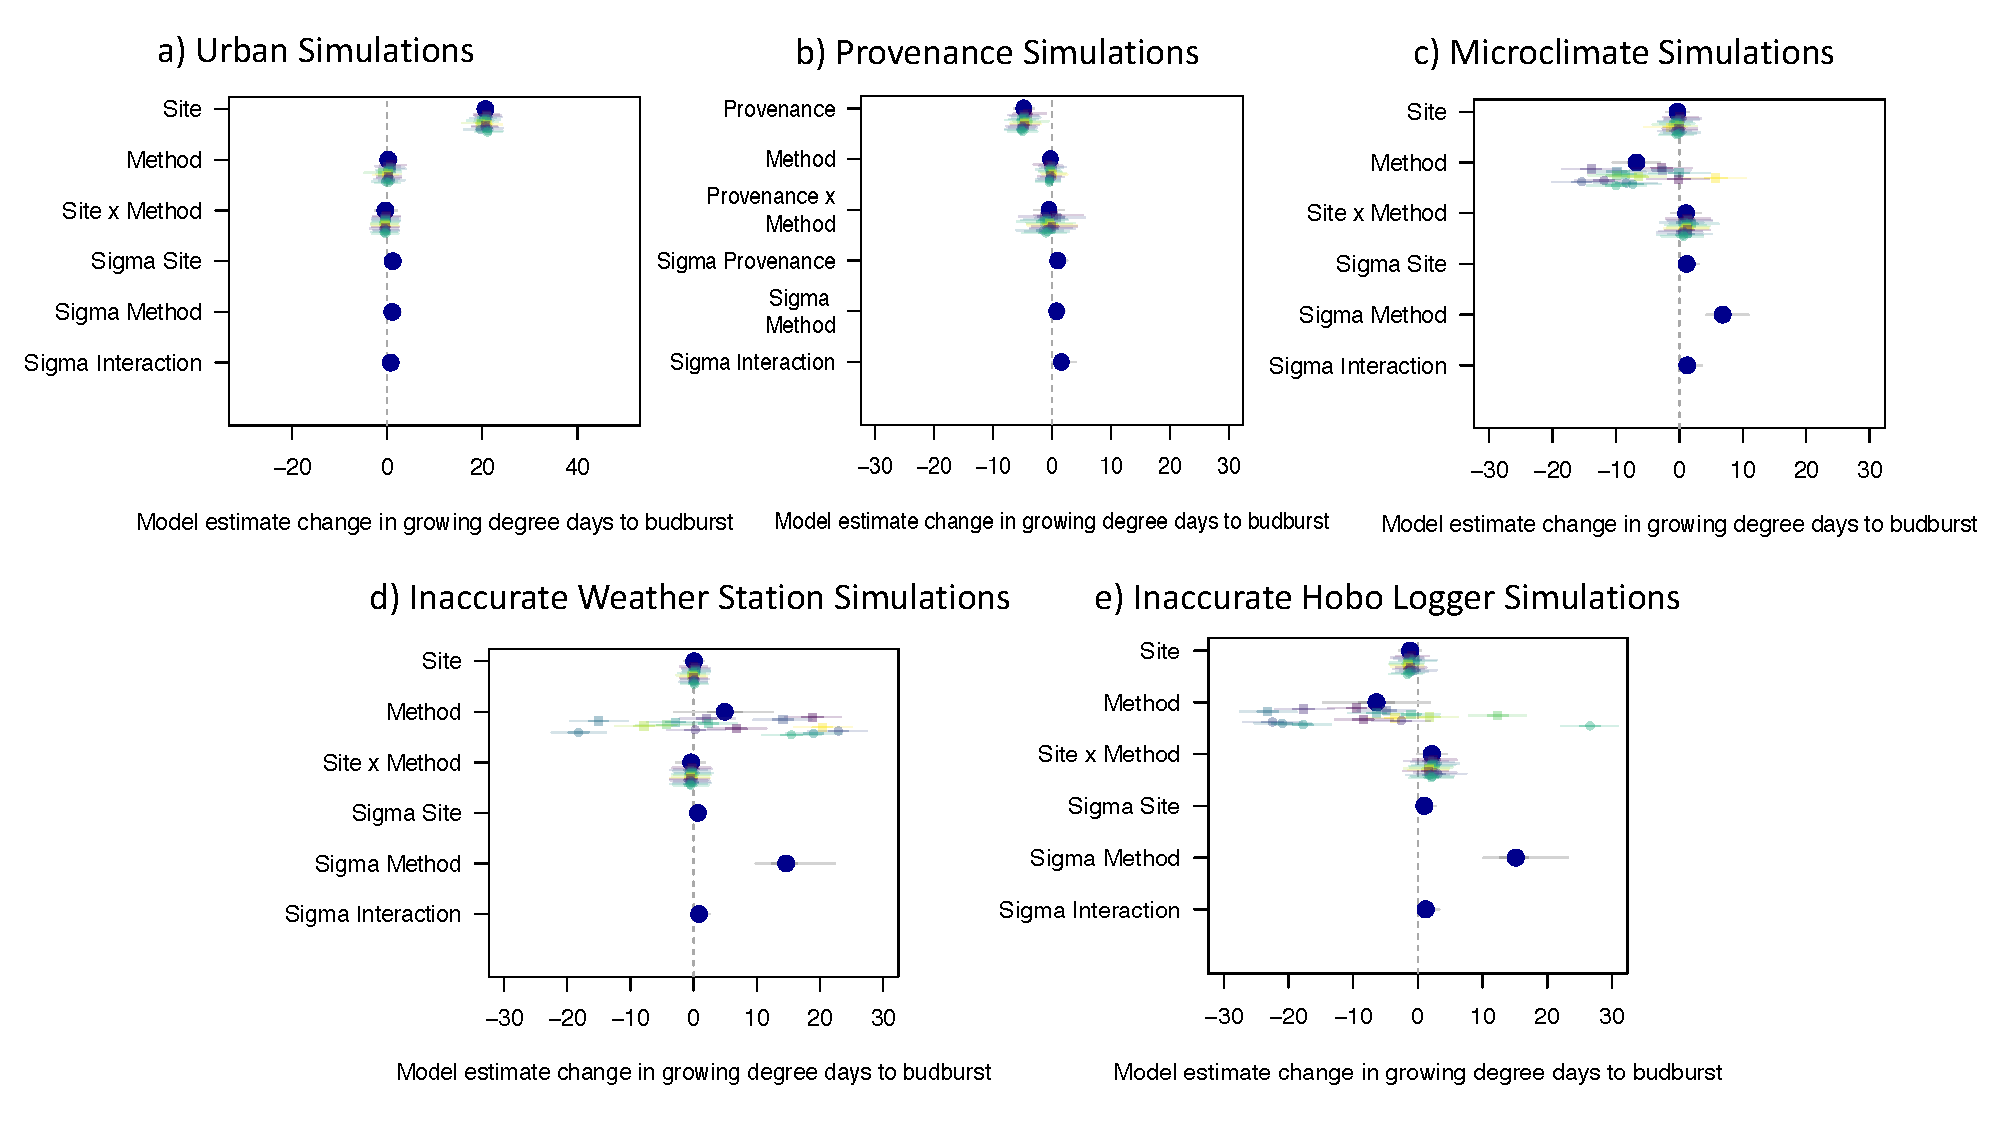
\includegraphics[width=16cm]{..//analyses/figures/muplot_sims.pdf}
\caption{ Simulations: we show (a) urban sites requiring more GDDs, (b) microclimate effects, (c) more northern provenance latitudes requiring fewer GDDs, (d) less accurate weather station data and (e) less accurate hobo logger data. We show the effects of site (urban versus rural) and method (weather station versus hobo loggers) in (a), (b), (d) and (e). The intercept represents the hobo logger data for the rural forested site. More positive values indicate more GDDs required for budburst whereas more negative values suggest fewer GDDs required. Dots and thin lines show means and 90\% uncertainty intervals and thick lines show 50\% uncertainty intervals. See Tables \ref{tab:urban}, \ref{tab:micros}, \ref{tab:prov}, \ref{tab:noisyws} and \ref{tab:noisyhobo} for full model output. } 
\label{fig:musims}
\end{figure}


\begin{figure}[H]
    \centering
    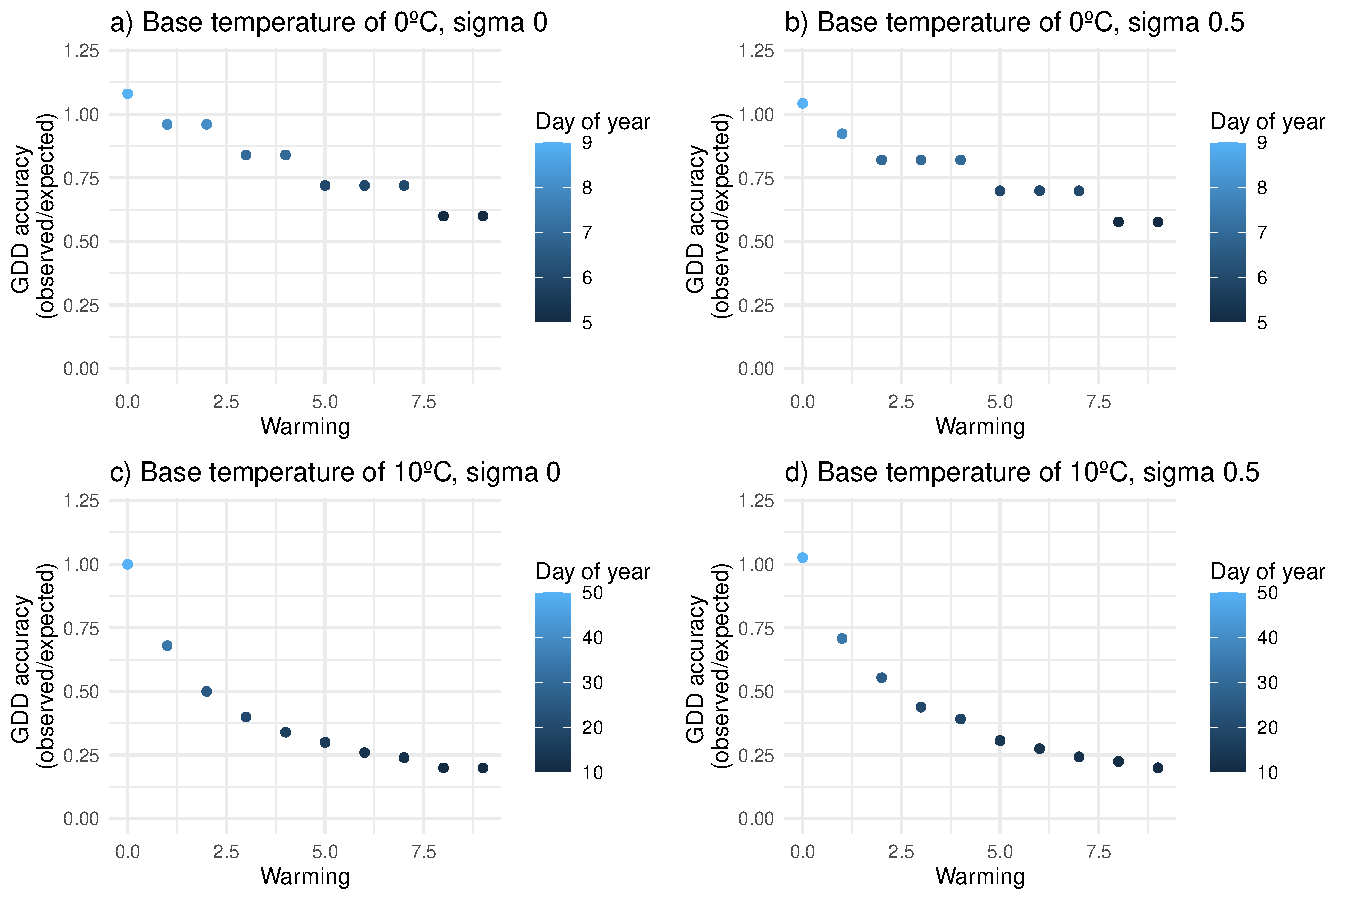
\includegraphics[height=8cm, width=12cm]{..//analyses/figures/gddratio_warming.pdf}
\caption{Using simulated data, we show how GDD measurement accuracy changes with warming (i.e., from 0$^{\circ}$C to 10$^{\circ}$C) using a base temperature of (a) 0$^{\circ}$C and a sigma of 0.1$^{\circ}$C, (b) 0$^{\circ}$C and a sigma of 1$^{\circ}$C, (c) 10$^{\circ}$C and a sigma of 0.1$^{\circ}$C and (d) 10$^{\circ}$C and a sigma of 1$^{\circ}$C. GDD accuracy is measured as the observed GDD divided by the expected GDD. Values closest to 1 are most accurate, with values deviating from 1 representing a percent change in inaccuracy (e.g., 1.1 is 10\% inaccurate). Observed GDD must always be equal to or greater than expected GDD in order for the threshold for budburst to be met, thus values will never be less than 1.}
\label{fig:warming}
\end{figure}


{\begin{figure} [H]
  \begin{center}
  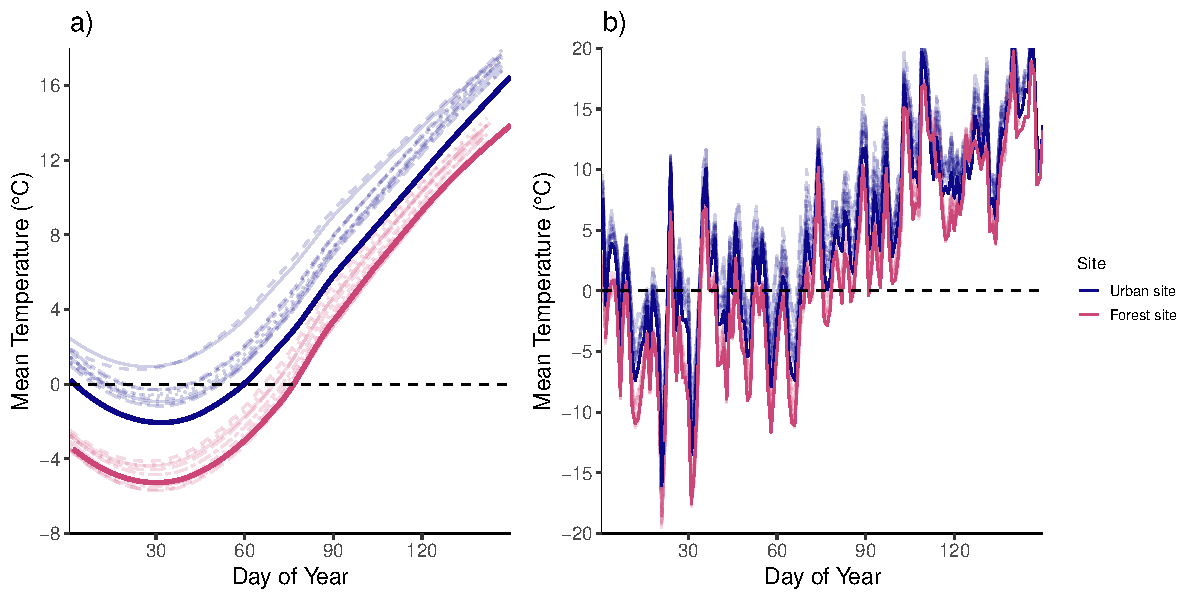
\includegraphics[width=12cm]{..//analyses/figures/climate_smoothdaily.pdf}
  \caption{Here we show a breakdown of the climate data across the two sites with darker lines representing weather station data and the lighter, more transparent lines of varying line types representing the hobo loggers: a) a series of smoothing splines of mean temperature with 90\% uncertainty interval and b) actual mean temperature.}\label{fig:clim}
  \end{center}
  \end{figure}}
  

\begin{figure}[H]
    \centering
    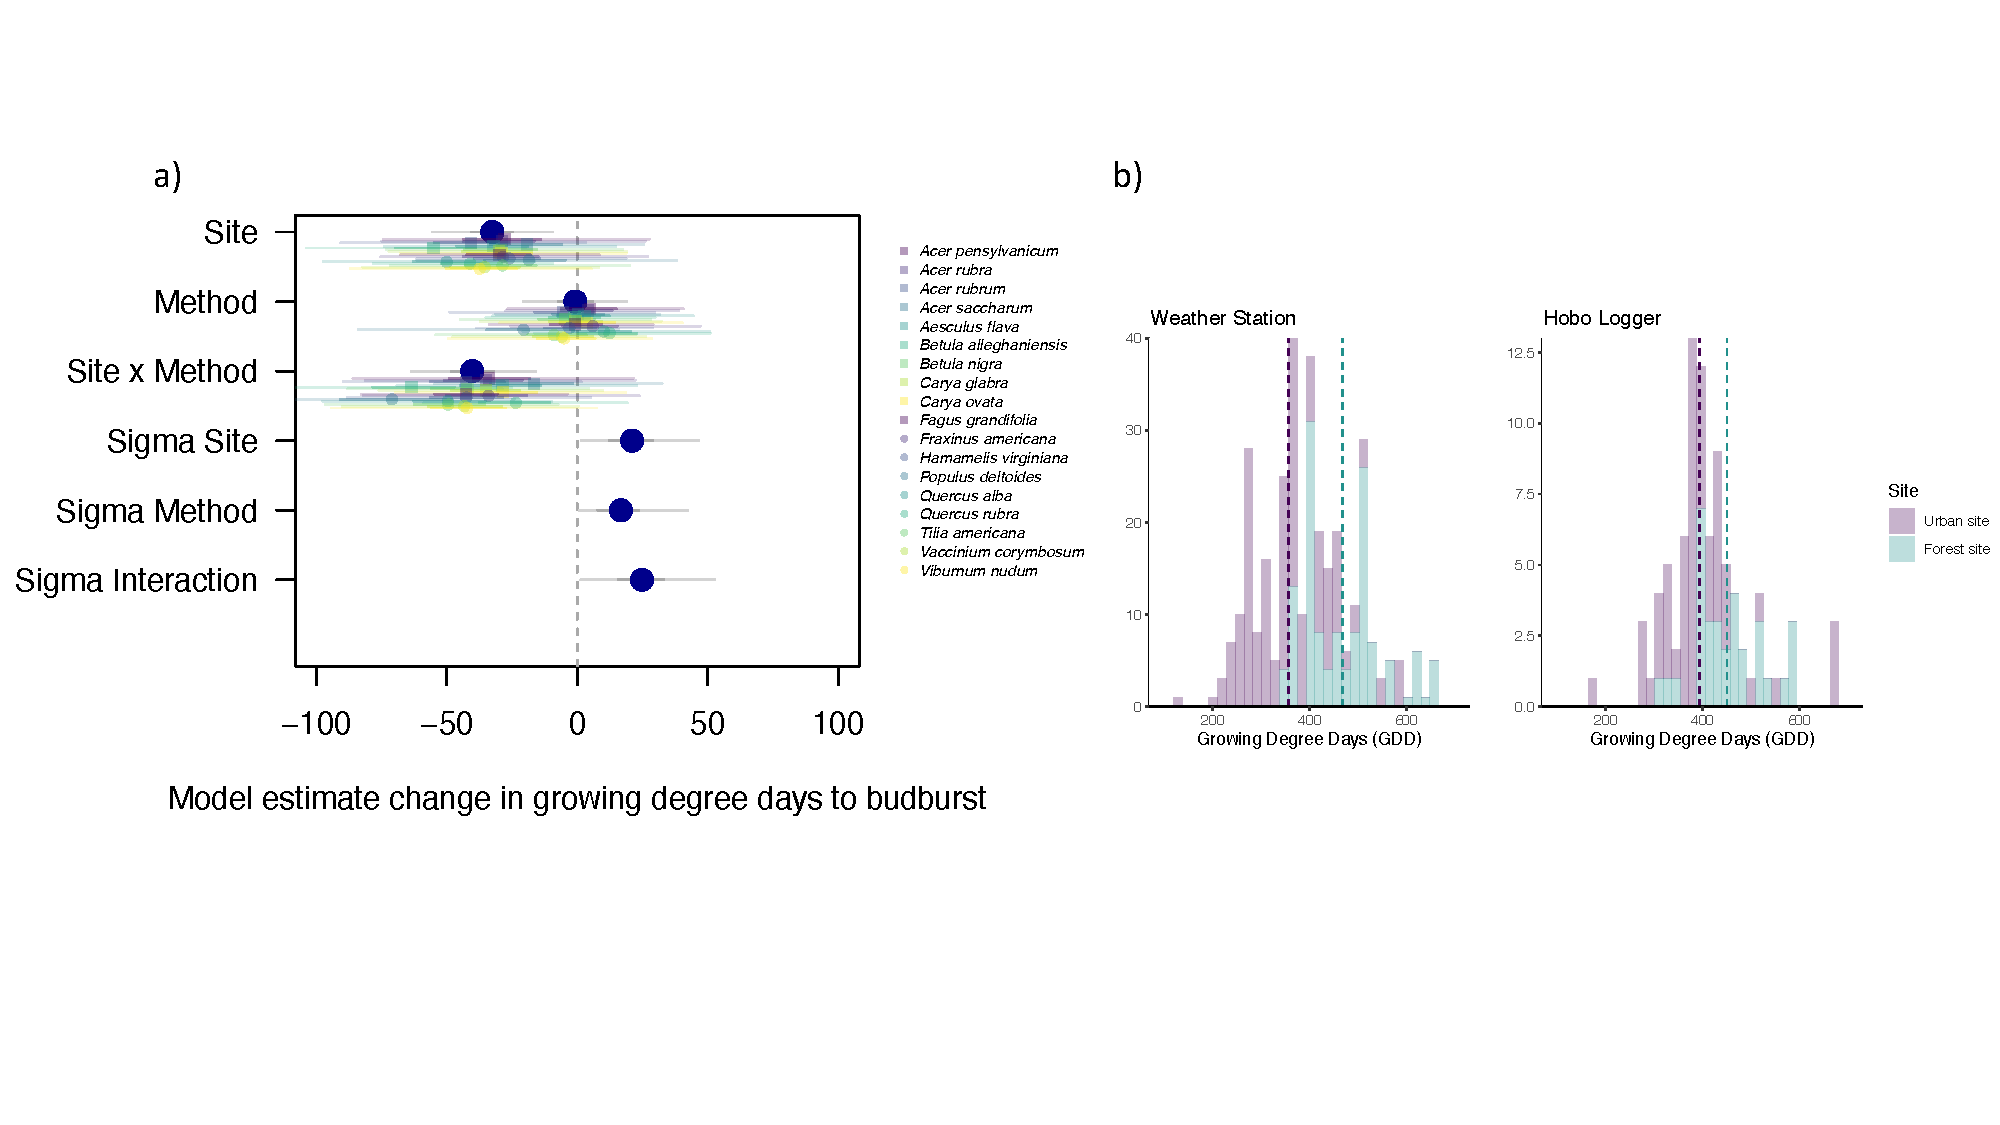
\includegraphics[width=16cm, trim=0cm 5cm 0cm 0cm,]{..//analyses/figures/muandgdd.pdf}
\caption{ Empirical Data: we show (a) the effects of site (urban versus rural) and climate data method (weather station versus hobo loggers) on GDDs until budburst. The intercept represents the hobo logger data for the rural forested site. More positive values indicate more GDDs are required for budburst whereas more negative values suggest fewer GDDs are required. Dots and thin lines show means and 90\% uncertainty intervals and thick lines show 50\% uncertainty intervals. See Table \ref{tab:real} for full model output. We also show (b) histograms of GDDs at the urban arboretum and rural forested site using weather station data and hobo logger data.}
\label{fig:real}
\end{figure}

\begin{figure}[H]
      \centering
      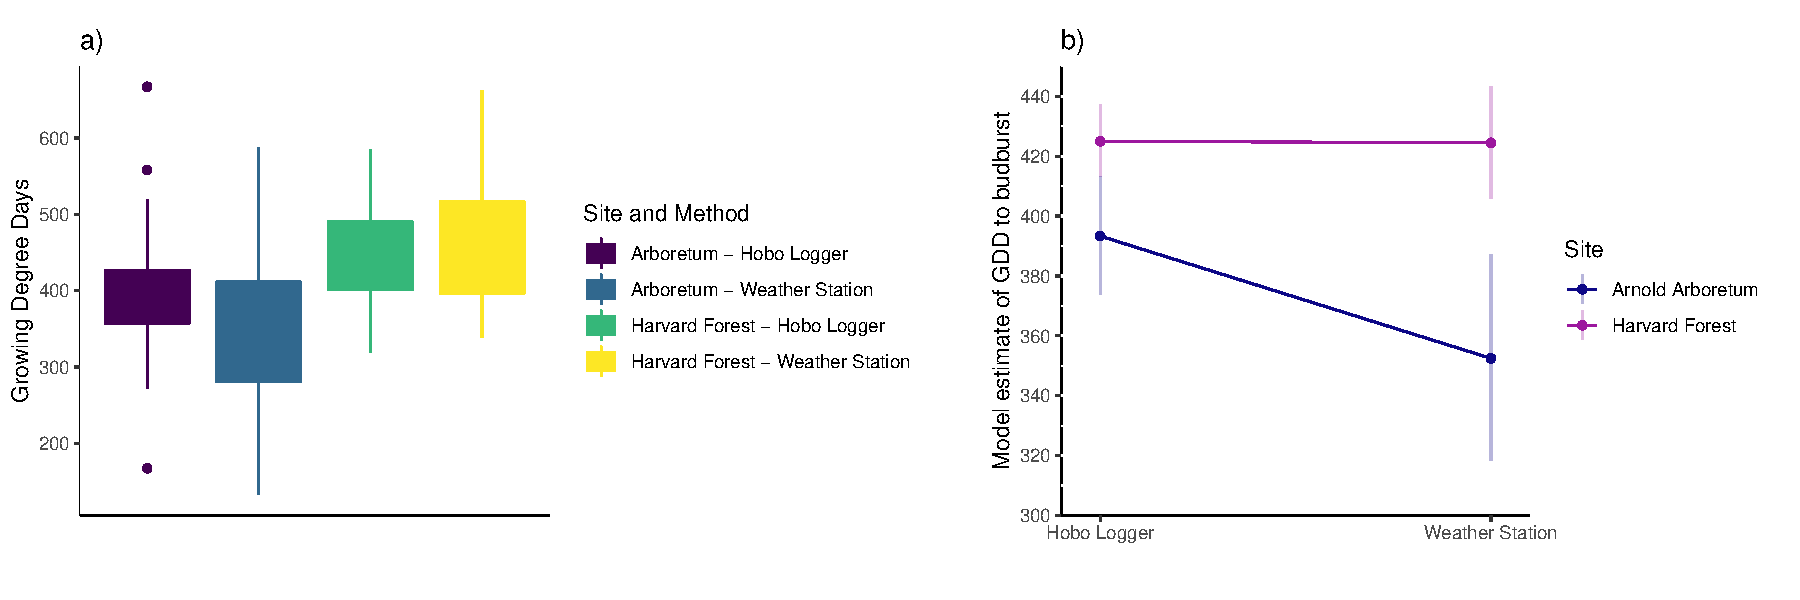
\includegraphics[width=16cm]{..//analyses/figures/gdd_interaction.pdf}
\caption{ We show effects of site (urban arboretum site versus forested rural site) by climate data method (weather station data versus hobo logger data) on GDDs until budburst (a) as a boxplot across each method and site combination using raw data and (b) using model output to show the mean estimates for each site and method with 50\% uncertainty intervals shown as error bars.}
\label{fig:interaction}
\end{figure}



  
  

\end{document}
